% $Id: TimeMgr_obj4.tex,v 1.3 2004/01/27 23:05:07 eschwab Exp $

%\section{Object Model}

In Time Manager, all times are internally represented and operated on as
integer seconds and rational integer fractional seconds.  Specific date and
time formats are available to the user at the interface level, where
conversions are performed.  So the user gets/sets Time Manager's
{\tt TimeIntervals} and {\tt Time} instants in familiar units of year, month,
day, hour, minutes, seconds, and sub-seconds in their various required
combinations.  Figure 4 shows an example of a user's ESM component querying
its clock for the current time in (yy, mm, dd, h, m, s) format.  First the
model invokes the {\tt Get()} method on its clock's current time,
{\tt CurrTime}.  Next, internally (transparent to the user), {\tt CurrTime}
invokes the {\tt ConvertToDate()} method on its associated calendar, Gregorian.
Gregorian, in turn, performs the requisite conversion of {\tt CurrTime}'s
internal representation of time (integer seconds and fractional seconds)
to a Gregorian date.  Note that the calendar object is a single instance
shared among all Time instants, as previously shown in Figures 1 and 2.

\begin{center}
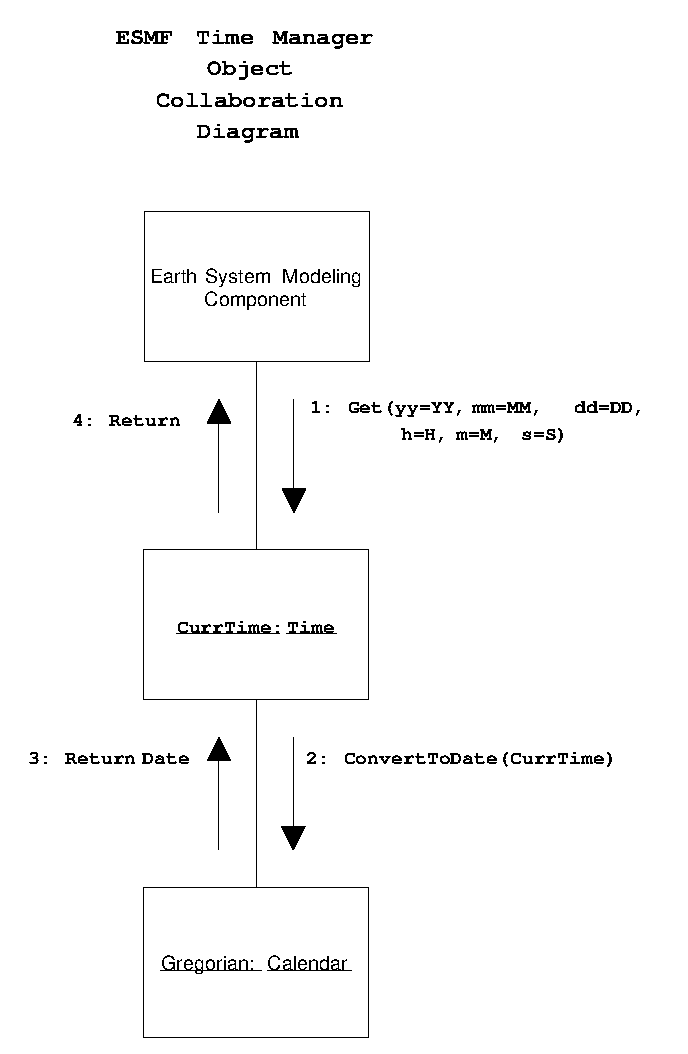
\includegraphics{TimeMgrOCD2.EPS}
   
Figure 4.  ESMF Time Manager Convert to Date Scenario
   
\end{center}
